%   ------------------------------------------------------------------------
\FloatBarrier
\subsection{Ferramenta de rotação}
\label{s.pixelLab.rotacao}

A ferramenta de rotação possui dois formatos: o componente chamado quick rotate (rotação rápida, em inglês) mostrado na Figura \ref{fig:pixelLabQuickRotateTela} no Apêndice \ref{ap.telasIA}, no qual, após ser selecionado pelo usuário, gera a nova imagem de acordo com o quanto foi arrastado horizontalmente (para definir o ângulo da rotação) e verticalmente (para o ângulo da inclinação) desde o momento do clique do mouse até a sua soltura; e a seção rotate (rotação, em inglês), que abre uma tela com várias configurações para gerar o personagem rotacionado, como pode ser visto na Figura \ref{fig:pixelLabRotateTela} no Apêndice \ref{ap.telasIA}. 

De acordo com a documentação, a ferramenta é melhor em fazer rotações pequenas, de forma que o resultado de uma rotação pode ser usado como a imagem inicial a ser rotacionada. Nesse método, porém, os erros são acumulados a cada rotação. Enquanto isso, há também a possibilidade de apenas fazer a rotação maior para evitar o acúmulo de erros, apesar de ser mais complicado para a IA.

Os testes dessa funcionalidade específica visavam criar a imagem do Pablo em side view, a partir do sprite mostrado na Figura \ref{fig:Pablo}.

Durante as primeiras tentativas, os resultados (Figura \ref{fig:pixelLabRotacao1}) não geraram nenhuma rotação, apenas fazendo deformações no personagem. Porém, foi descoberto em testes posteriores que, para a geração de um bom resultado, o sprite deve estar centralizado no meio da tela, como pode ser visto na Figura \ref{fig:pixelLabRotCompara}.


\begin{figure}[htbp]
    \centering
    \caption{\small Comparação rotação 90 graus no Pixel Lab}
    \label{fig:pixelLabRotCompara}
    \begin{subfigure}{0.45\linewidth}
        \centering
        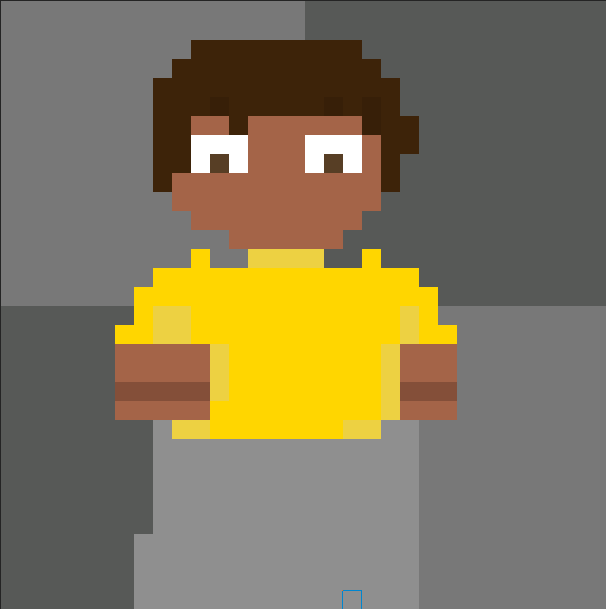
\includegraphics[width=0.5\linewidth]{figs/pixelLab/dia1/resultado rotacao 2.PNG}
        \caption{\small Resultado a partir do sprite inicialmente no canto esquerdo da tela}
        \label{fig:pixelLabRotComparaCanto}
    \end{subfigure}
    \begin{subfigure}{0.45\linewidth}
        \centering
        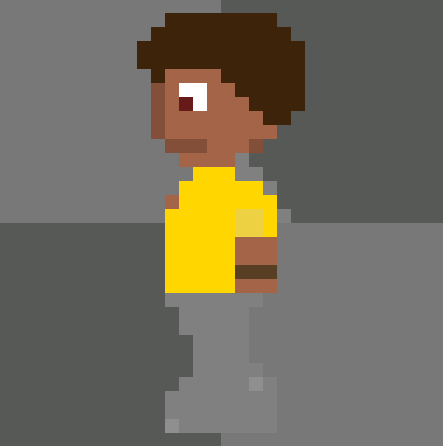
\includegraphics[width=0.5\linewidth]{figs/pixelLab/dia2/rot90res1.PNG}
        \caption{\small Resultado a partir do sprite inicialmente no centro da tela}
        \label{fig:pixelLabRotComparaCentro}
    \end{subfigure}

    \legend{\small Fonte: Elaborada pela autora, utilizando a ferramenta Pixel Lab.}
\end{figure}

Dessa forma, os testes prosseguiram posicionando a imagem corretamente, gerando rotações consistentes com o personagem e o estilo, porém com algumas deformações. Analisando os resultados, foi possível perceber que a ferramenta apresenta uma dificuldade na região onde ficaria o nariz, gerando essa parte com mais imperfeições. Além disso, foi notado que existe um processo para conseguir usar somente as cores da imagem de referência:
\begin{itemize}
    \item A imagem é gerada sem restrição nas cores (Figura \ref{fig:pixelLabProcesso1});
    \item A imagem é recriada com tons de cores similares aos da paleta do sprite original, não possuindo restrição no número de tonalidades (Figura \ref{fig:pixelLabProcesso2}); e
    \item O fundo é removido e cada uma das cores é igualada à mais semelhante da paleta original (Figura \ref{fig:pixelLabProcesso3}).
\end{itemize}

\begin{figure}[htbp]
    \centering
    \caption{\small Etapas do processamento da geração de imagem no Pixel Lab}
    \label{fig:pixelLabRotProcesso}
    \begin{subfigure}{0.32\linewidth}
        \centering
        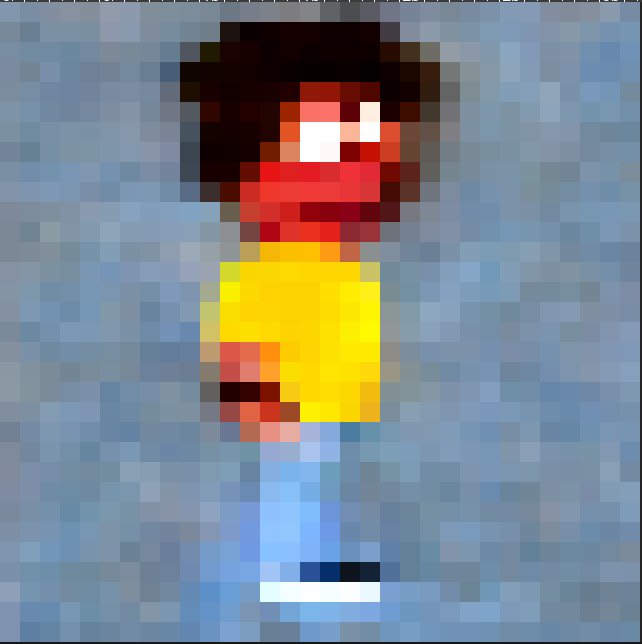
\includegraphics[width=1\linewidth]{figs/pixelLab/dia2/cores_tudo_estranha.PNG}
        \caption{\small Imagem da rotação no início do processamento}
        \label{fig:pixelLabProcesso1}
    \end{subfigure}
    \begin{subfigure}{0.32\linewidth}
        \centering
        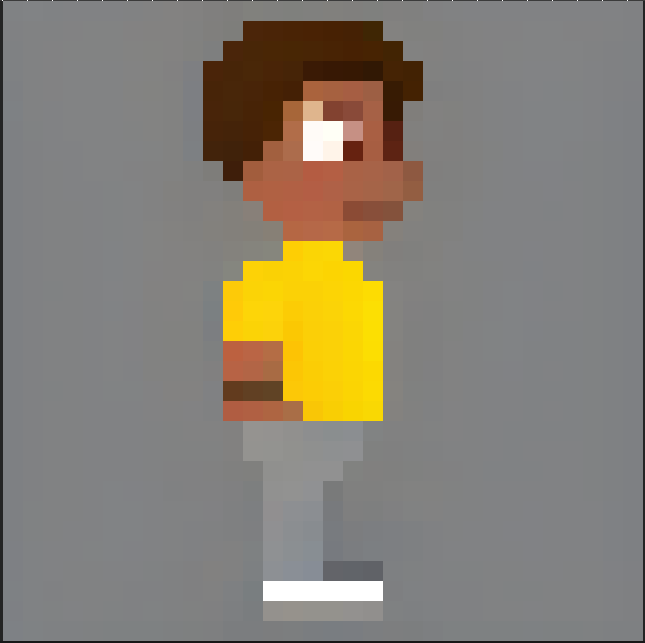
\includegraphics[width=1\linewidth]{figs/pixelLab/dia2/perna_antes_de_sumir.PNG}
        \caption{\small Imagem da rotação no meio do processamento, com cores mais parecidas às do sprite original, porém com mais tons}
        \label{fig:pixelLabProcesso2}
    \end{subfigure}
    \begin{subfigure}{0.32\linewidth}
        \centering
        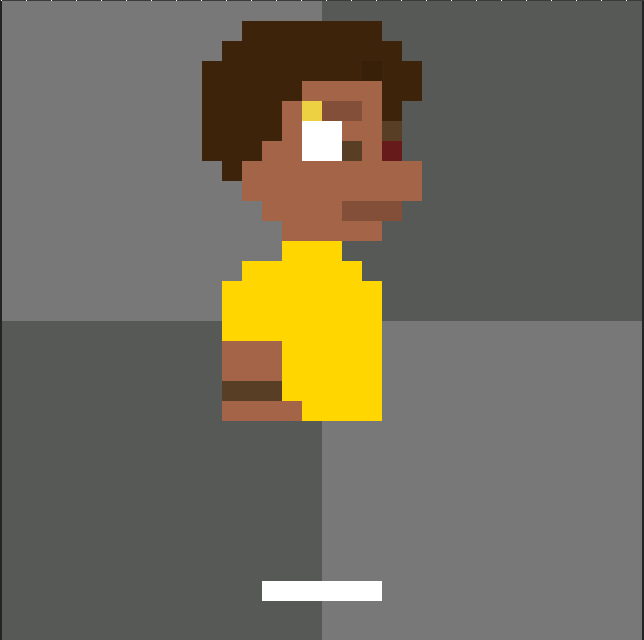
\includegraphics[width=1\linewidth]{figs/pixelLab/dia2/demonstrar_perna_sumindo.PNG}
        \caption{\small Imagem da rotação após o processamento, com cores igualadas ao do sprite original, porém removendo a perna}
        \label{fig:pixelLabProcesso3}
    \end{subfigure}

    \legend{\small Fonte: Elaborada pela autora, utilizando a ferramenta Pixel Lab.}
\end{figure}

Esse processo faz com que nem todas as características do personagem possuam a cor correta, além de muitas vezes causar o desaparecimento da calça por reconhecê-la como parte do fundo, já que as cores são semelhantes. Esses detalhes são mostrados na Figura \ref{fig:pixelLabRotComparaCor}. A demonstração completa dos testes é encontrada nas Figuras \ref{fig:pixelLabRotacao2} a \ref{fig:pixelLabRotacao4}.

\begin{figure}[htbp]
    \centering
    \caption{\small Comparação de cores entre o sprite original e o resultado gerado no Pixel Lab}
    \label{fig:pixelLabRotComparaCor}
    \begin{subfigure}{0.45\linewidth}
        \centering
        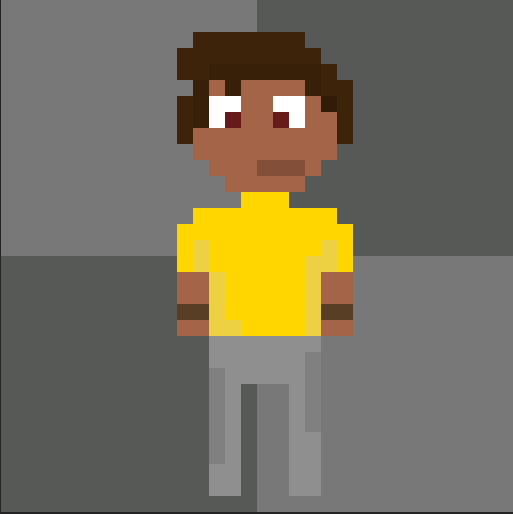
\includegraphics[width=1\linewidth]{figs/pixelLab/dia2/sprite_centro.PNG}
        \caption{\small Imagem original com olho castanho escuro e calça completa}
        \label{fig:pixelLabRotComparaCorA}
    \end{subfigure}
    \begin{subfigure}{0.45\linewidth}
        \centering
        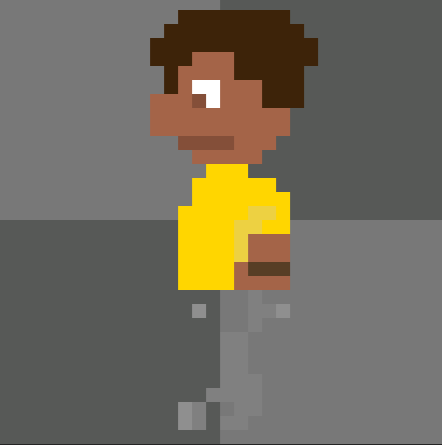
\includegraphics[width=1\linewidth]{figs/pixelLab/dia2/rot90res2.PNG}
        \caption{\small Resultado com olho castanho claro e parte da calça faltando}
        \label{fig:pixelLabRotComparaCorB}
    \end{subfigure}

    \legend{\small Fonte: Elaborada pela autora, utilizando a ferramenta Pixel Lab.}
\end{figure}

Na bateria seguinte de testes, foram realizados ajustes finos em algumas das imagens geradas de 45°, com o objetivo de gerar novamente o personagem em 90°, em uma tentativa de contornar o problema dos erros cumulativos. Como a ferramenta possui um editor integrado, é extremamente fácil e eficiente corrigir erros, diferente do que aconteceu em outras ferramentas. As edições feitas podem ser consultadas na Figura \ref{fig:pixelLabAjusteFino1} abaixo e na Figura \ref{fig:pixelLabAjusteFino2} no Apêndice \ref{ap.telasIA}.

\begin{figure}[htbp]
    \centering
    \caption{\small Ajuste fino no resultado da rotação de 45 graus no Pixel Lab}
    \label{fig:pixelLabAjusteFino1}
    \begin{subfigure}{0.45\linewidth}
        \centering
        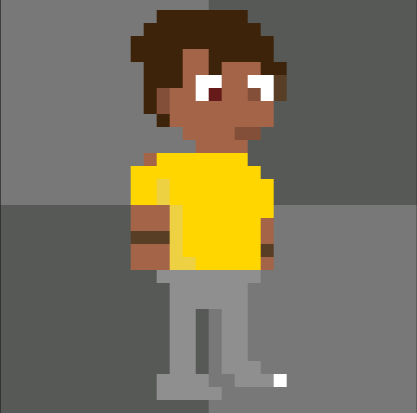
\includegraphics[width=1\linewidth]{figs/pixelLab/dia2/rot45res4.PNG}
        \caption{\small Antes da edição}
        \label{fig:pixelLabAjusteFino1a}
    \end{subfigure}
    \begin{subfigure}{0.45\linewidth}
        \centering
        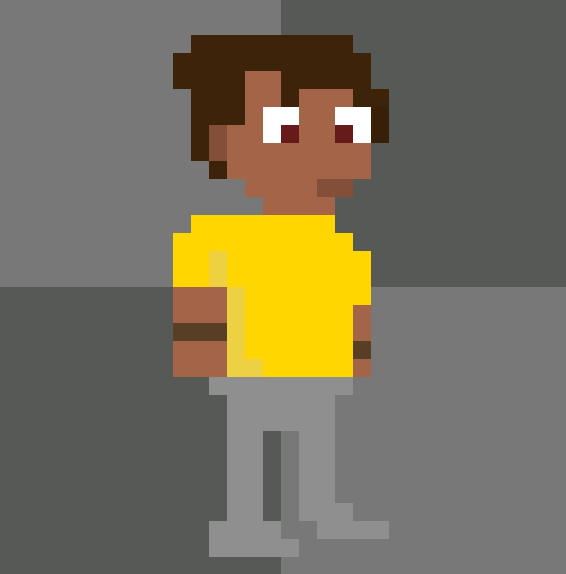
\includegraphics[width=1\linewidth]{figs/pixelLab/dia2/fix_teste_4.PNG}
        \caption{\small Após edição}
        \label{fig:pixelLabAjusteFino1b}
    \end{subfigure}

    \legend{\small Fonte: Elaborada pela autora, utilizando a ferramenta Pixel Lab.}
\end{figure}

Após esse ajuste, mais testes foram feitos, porém os resultados gerados (Figuras \ref{fig:pixelLabRotacao6} a \ref{fig:pixelLabRotacao9} no Apêndice \ref{ap.telasIA}) não mostraram nenhuma melhora significativa, aparentando possuir mais deformações e imprecisões do que anteriormente. Isso pode ser melhor notado na Figura \ref{fig:pixelComparaAjuste}.

\begin{figure}[htbp]
    \centering
    \caption{\small Comparação de resultados antes e depois do ajuste fino}
    \label{fig:pixelComparaAjuste}
    \begin{subfigure}{0.45\linewidth}
        \centering
        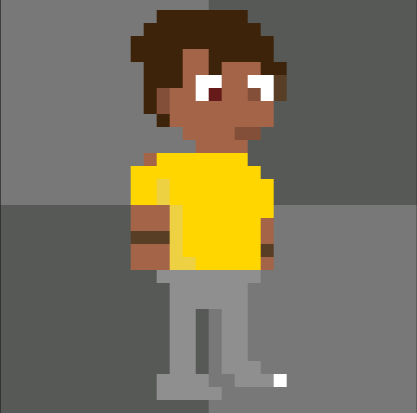
\includegraphics[width=1\linewidth]{figs/pixelLab/dia2/rot45res4.PNG}
        \caption{\small Resultado gerado a partir da imagem sem o ajuste fino, com uma deformação na região do nariz e boca e erros e pequenos erros na proporção do corpo}
        \label{fig:pixelComparaAjusteAntes}
    \end{subfigure}
    \begin{subfigure}{0.45\linewidth}
        \centering
        
\includegraphics[width=1\linewidth]{figs/pixelLab/dia2/rot45fix3res2.PNG}
        \caption{\small Resultado gerado a partir da imagem com o ajuste fino, onde apenas a cabeça do sprite gerado aparenta estar rotacionada e com um deformação no olho}
        \label{fig:pixelComparaAjusteDepois}
    \end{subfigure}

    \legend{\small Fonte: Elaborada pela autora, utilizando a ferramenta Pixel Lab.}
\end{figure}

Considerando a falha na abordagem anterior, uma nova estratégia foi montada considerando uma das opções de customização que a ferramenta rotate oferece: init image (imagem de inicialização, em inglês). Essa funcionalidade permite ao usuário indicar uma imagem para guiar a IA em como deve ficar o resultado final, tendo uma variável associada chamada init image strength (força da imagem de inicialização, em inglês) para indicar o quanto essa inicialização deve ser utilizada. 

Na primeira instância, o melhor resultado gerado do personagem em side view na ferramenta é usado como imagem de inicialização, como pode ser visto na Figura \ref{fig:pixelLabRotInit} no Apêndice \ref{ap.telasIA}.

Os resultados gerados (Figura \ref{fig:pixelLabRotacao10} no Apêndice \ref{ap.telasIA}) apresentaram uma melhor performance comparada aos sprites gerados sem nenhuma imagem de inicialização, porém demonstraram erros na região da calça, o que também pode ser visto na imagem de inicialização, apesar de com menos intensidade. Devido a esse fator, foi feita uma edição na init image, que pode ser vista na Figura \ref{fig:pixelLabAjusteFino3}.

\begin{figure}[htbp]
    \centering
    \caption{\small Edição no resultado da rotação de 90 graus no Pixel Lab}
    \label{fig:pixelLabAjusteFino3}
    \begin{subfigure}{0.45\linewidth}
        \centering
        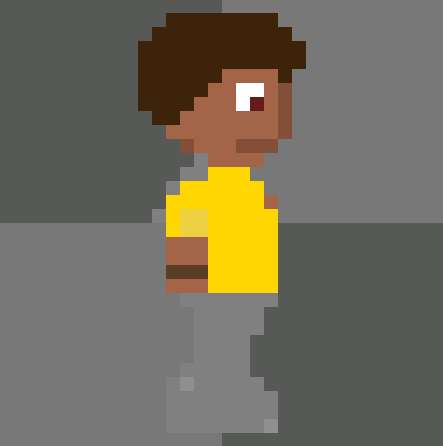
\includegraphics[width=1\linewidth]{figs/pixelLab/dia2/init.PNG}
        \caption{\small Antes da edição}
        \label{fig:pixelLabAjusteFino3a}
    \end{subfigure}
    \begin{subfigure}{0.45\linewidth}
        \centering
        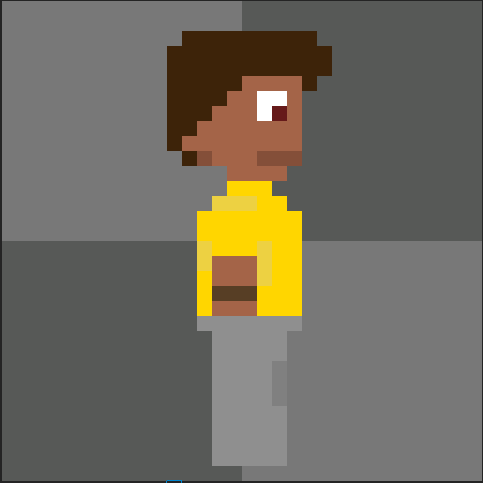
\includegraphics[width=1\linewidth]{figs/pixelLab/dia2/fix_init_1.PNG}
        \caption{\small Após edição}
        \label{fig:pixelLabAjusteFino3b}
    \end{subfigure}

    \legend{\small Fonte: Elaborada pela autora, utilizando a ferramenta Pixel Lab.}
\end{figure}

Analisando as imagens geradas (Figura \ref{fig:pixelLabRotacao11} no Apêndice \ref{ap.telasIA}) ainda não foi encontrado nenhum resultado satisfatório, com todos os sprites gerados sem as pernas.

Reavaliando todos os resultados, apesar da ferramenta quase ter gerado resultados satisfatórios, nenhum dos sprites alcança os padrões de qualidade para sua aplicação no jogo. Porém, a Figura \ref{fig:pixelLabAjusteFino2c} no Apêndice \ref{ap.telasIA} e a Figura  \ref{fig:pixelLabAjusteFino3b} foram usadas como referência para fornecer um contexto maior do personagem nas ferramentas ChatGPT (detalhada na Seção \ref{s.chatGPT}) e GeminiPro (detalhada na Seção \ref{s.ferramentaB}).

A análise da funcionalidade de rotação indica que, embora a ferramenta não elimine a necessidade de intervenção manual, ela otimiza o processo de criação. Os resultados, embora exijam edições e ajustes finos para atingir a qualidade desejada, fornecem uma base com alta consistência e fidelidade que auxilia na produção dos sprites do personagem.

